% !TeX spellcheck = en_US
\section{Problem 6}

The neural network described in Problem 6 is a simple NN with 2 inputs and 1 neuron. 
The difference with a simple fully connected NN is that the neuron has a third pseudo-input which is the product of both inputs $p_1$ and $p_2$.
This NN is shown in figure~\ref{fig:prob6_nn}.

\begin{figure}[htpb]
	\centering
	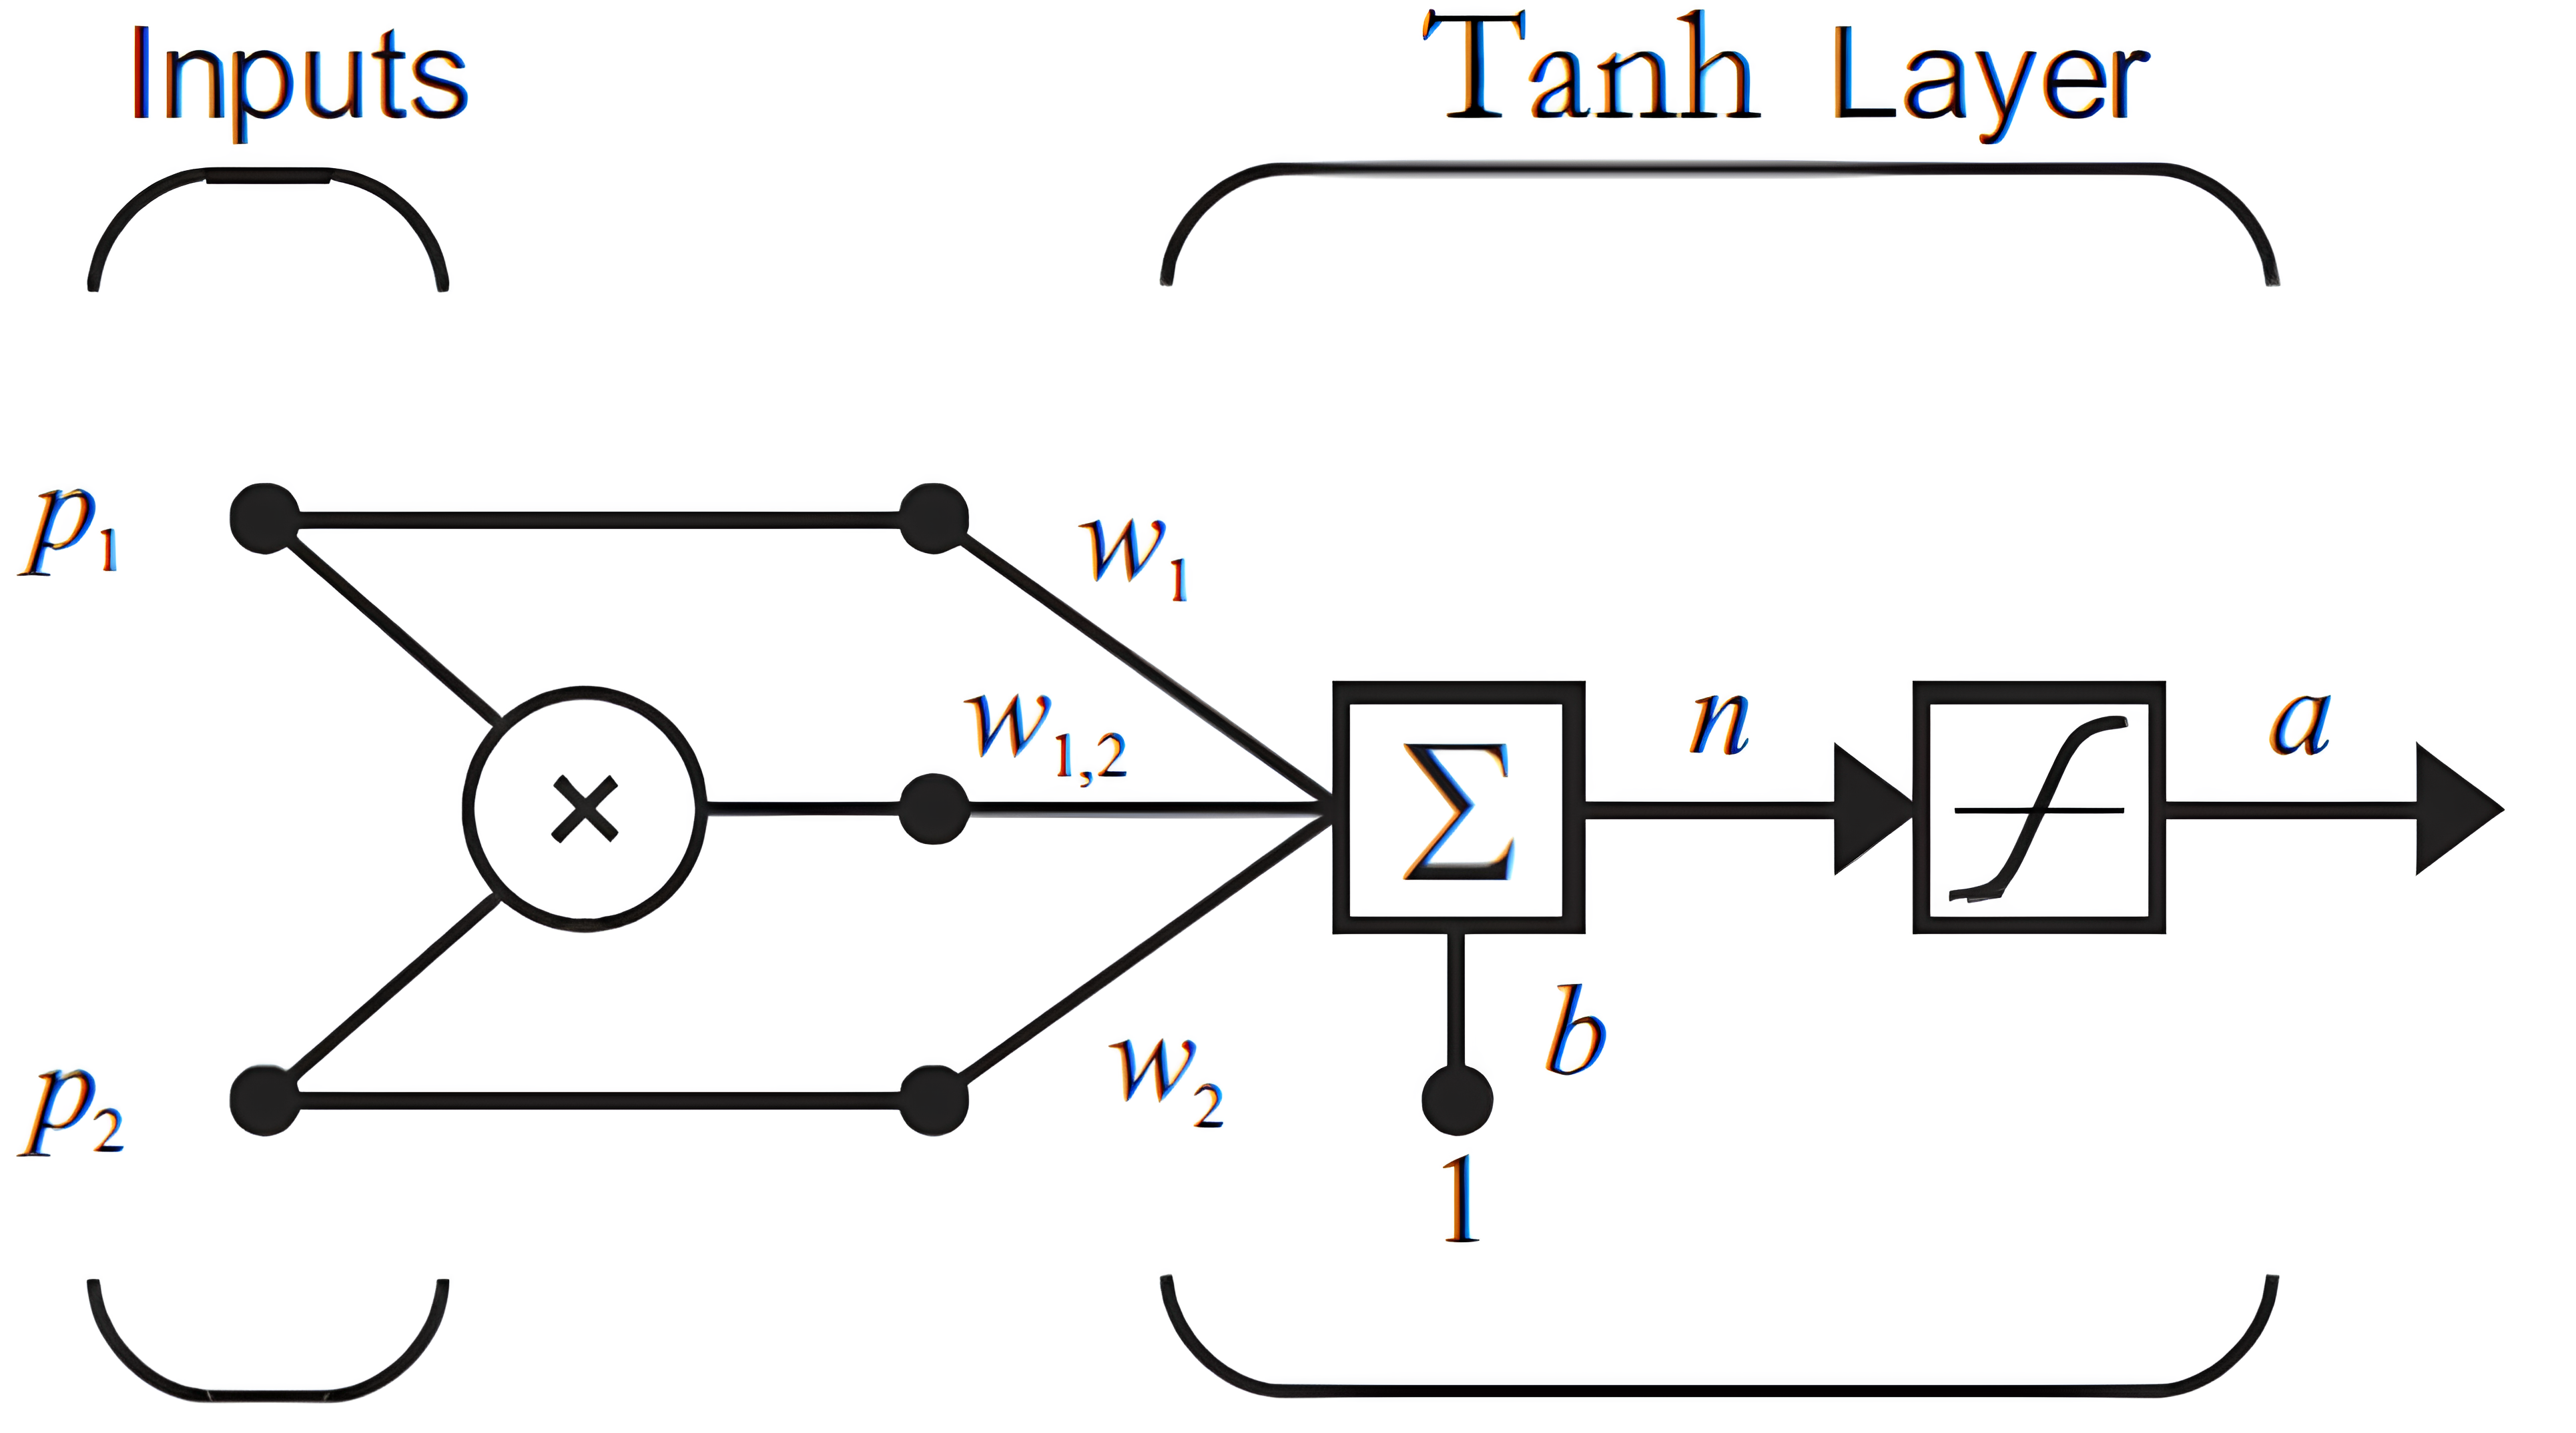
\includegraphics[width=0.4\textwidth]{../Problem 6/prob6_nn.png}
	\caption{The NN described in Problem 6}
	\label{fig:prob6_nn}
\end{figure}

\subsection{Learning rule}

The neural network's output is described by the following function:
\[
n = w_1 \cdot p_1 + w_2 \cdot p_2 + w_{1,2} \cdot \left(p_1 \cdot p_2\right) + b
\]

Assuming we have MSE (\textit{Mean Squared Error}), then loss function is the following $L = 1/2 \left( target - a\right)^2$.
It's derivative is $\dfrac{\theta L}{\theta a} = (a-target)$.

Since $a$ is the output of the $tanh$ activation function applied to $n$, $a$'s derivative in respect to $n$ is
$\dfrac{da}{dn} = 1 - tanh^2 \left(n\right)$.

For weights $w_1, w_2, w_{1,2}$ and bias $b_1$, the gradients are:
\[
\begin{array}{l}
	\dfrac{\theta n}{\theta w_1} = p_1 \\[3mm]
	\dfrac{\theta n}{\theta w_2} = p_2 \\[3mm]
	\dfrac{\theta n}{\theta w_{1,2}} = p_1 \cdot p_2 \\ [3mm]
	\dfrac{\theta n}{\theta b_1} = 1
\end{array}
\]

Using the chain rule, gradients of loss function with respect to weights and bias are:
\[
\begin{array}{l}
	\dfrac{\theta L}{\theta w_1} = \dfrac{\theta L}{\theta a} \cdot \dfrac{da}{dn} \cdot \dfrac{\theta n}{\theta w_1} \\[3mm]
	\dfrac{\theta L}{\theta w_2} = \dfrac{\theta L}{\theta a} \cdot \dfrac{da}{dn} \cdot \dfrac{\theta n}{\theta w_2} \\[3mm]
	\dfrac{\theta L}{\theta w_{1,2}} = \dfrac{\theta L}{\theta a} \cdot \dfrac{da}{dn} \cdot \dfrac{\theta n}{\theta w_{1,2}} \\[3mm]
	\dfrac{\theta L}{\theta b_1} = \dfrac{\theta L}{\theta a} \cdot \dfrac{da}{dn} \cdot \dfrac{\theta n}{\theta b_1} \\[3mm]
\end{array}
\]

Finally, update rules for weights and biases are:
\[
\begin{aligned}
	w_1 &= w_1 - a \dfrac{\theta L}{\theta w_1}\\
	w_2 &= w_2 - a \dfrac{\theta L}{\theta w_2}\\
	w_{1,2} &= w_{1,2} - a \dfrac{\theta L}{\theta w_{1,2}}\\
	w_1 &= b_1 - a \dfrac{\theta L}{\theta b_1}
\end{aligned}
\]


\subsection{Perform iteration}
The file \verb|prob6.m| contains an implementation of this neural network as well as the learning rule we created above.
Using as initial values the ones found in table~\ref{table:prob6_initial_values},
we get the new ones found in table~\ref{table:prob6_final_values} after one iteration of the steepest descend algorithm.

\begin{minipage}{0.47\textwidth}
	\centering
	\[
		\begin{tblr}{hlines, vlines, colspec={cc}}
			\textbf{Variable} & \textbf{Value}\\
			w_1 & 1 \\
			w_2 & -1 \\
			w_{1,2} & 0.5\\
			b_1 & 1\\
			p_1 & 0 \\
			p_2 & 1 \\
			target & 0.75 
		\end{tblr}
	\]
	\captionof{table}{Neural network's initial values}
	\label{table:prob6_initial_values}
\end{minipage}\hfill
\begin{minipage}{0.47\textwidth}
	\centering
	\[
		\begin{tblr}{hlines, vlines, colspec={cc}}
			\textbf{Variable} & \textbf{Value}\\
			w_1 & 1 \\
			w_2 & -0.25 \\
			w_{1,2} & 0.5\\
			b_1 & 1.75\\
			p_1 & 0 \\
			p_2 & 1 \\
			outputs & 0.9051
		\end{tblr}
	\]
	\captionof{table}{NN's values after 1 iteration}
	\label{table:prob6_final_values}
\end{minipage}